% !TEX root = ./trigger.tex
\section{Physics triggers}


%%%%%%%%   Overview   %%%%%%%%


%\begin{figure}[htp]
%\begin{center}
%\centering
%\includegraphics[width=8cm, angle=270]{clas12-design.pdf}
%\caption{CLAS 12 detector and its subsystems.}
%\label{fig:CLAS12}
%\end{center}
%\end{figure}

The CLAS12 detector  has been designed to study the interactions of electrons and photons with nucleons and nuclei at high luminosity. 
The CLAS12 trigger system is providing trigger signals for these processes. 
Any detectors with Flash Analog to Digital Converter (FADC) front-end electronics may participate in the trigger event selection.  In addition, track reconstruction by the drift chambers at the trigger level is used to select events with charge particles in the final state. 
%(see Fig.~\ref{fig:CLAS12}). 
The trigger firmware has access to  the following detectors:
\begin{itemize}
\item High Threshold Cherenkov Counter (HTCC)
\item Drift Chambers (DC)
\item Low Threshold Cherenkov Counter (LTCC)
\item Time of Flight System (TOF)
\item Preshower Calorimeter (PCAL)
\item Electromagnetic Calorimeter (EC).
%\item Silicon Vertex Detector (SVT)
\item Central Time of Flight (CTOF)
\item Central Neutron Detector (CND)
\item Forward Tagger (FT)
\end{itemize}

\subsection{Electron Trigger}
The electron trigger is designed to select the inclusive electron scattering out of the CLAS12 targets:
\begin{equation}
e(p,n,A)\rightarrow e^\prime X.
\label{eqn:electron}
\end{equation}
\noindent
The trigger  selects  events with the at least one scattered  electron detected by the forward detectors.
Searching for the electrons is performed  in all six CLAS12 sectors in parallel. The final electron trigger is  a simple "OR" of the six sector trigger signals.
High Threshold Cherenkov Counter,  Preshower Calorimeter,   Electromagnetic Calorimeter and Drift Chambers are participating in the generation of the trigger decision.

\begin{figure}[htp]
\begin{center}
\centering
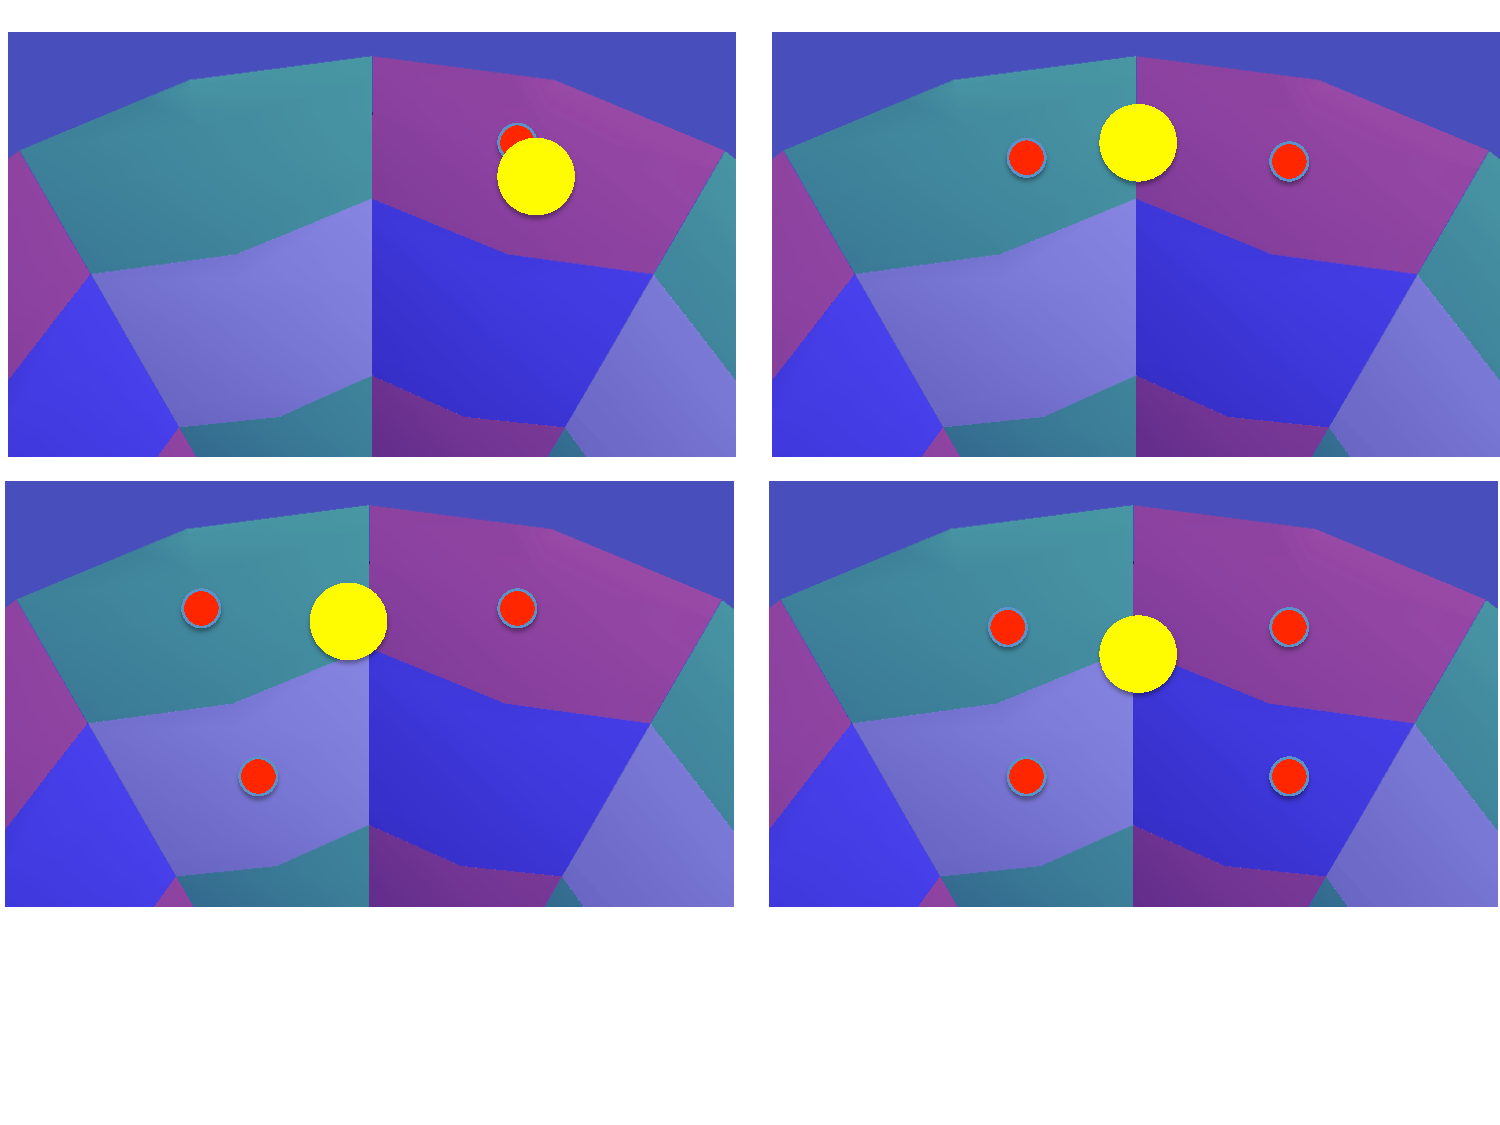
\includegraphics[width=8cm]{img/multiHits.pdf}
\caption{Hits registered by HTCC (red circles) and reconstructed cluster position (yellow). They coincide for one hit clusters (top left plot) which has the lowest resolution.}
\label{fig:multihitHTCC}
\end{center}
\end{figure} 

HTCC  was specially designed to discriminate electrons from other charge particles. 
The detector has to be calibrated before the experiment in terms of number of photoelectrons. The HTCC trigger firmware
is searching for the clusters in parallel at each of six CLAS12 sectors and is calculating the total number of photoelectrons  detected by HTCC. The cluster may include one, two, three or maximum four PMT's signals collecting the Cherenkov light from the adjacent mirrors as shown in  Fig.~\ref{fig:multihitHTCC}. The minimum number of  photoelectrons in the cluster  is one of the main electron trigger parameters. Usually this parameter equals 1-2 photoelectrons depending on the experiment requirements.
\begin{figure}[htp]
\begin{center}
\centering
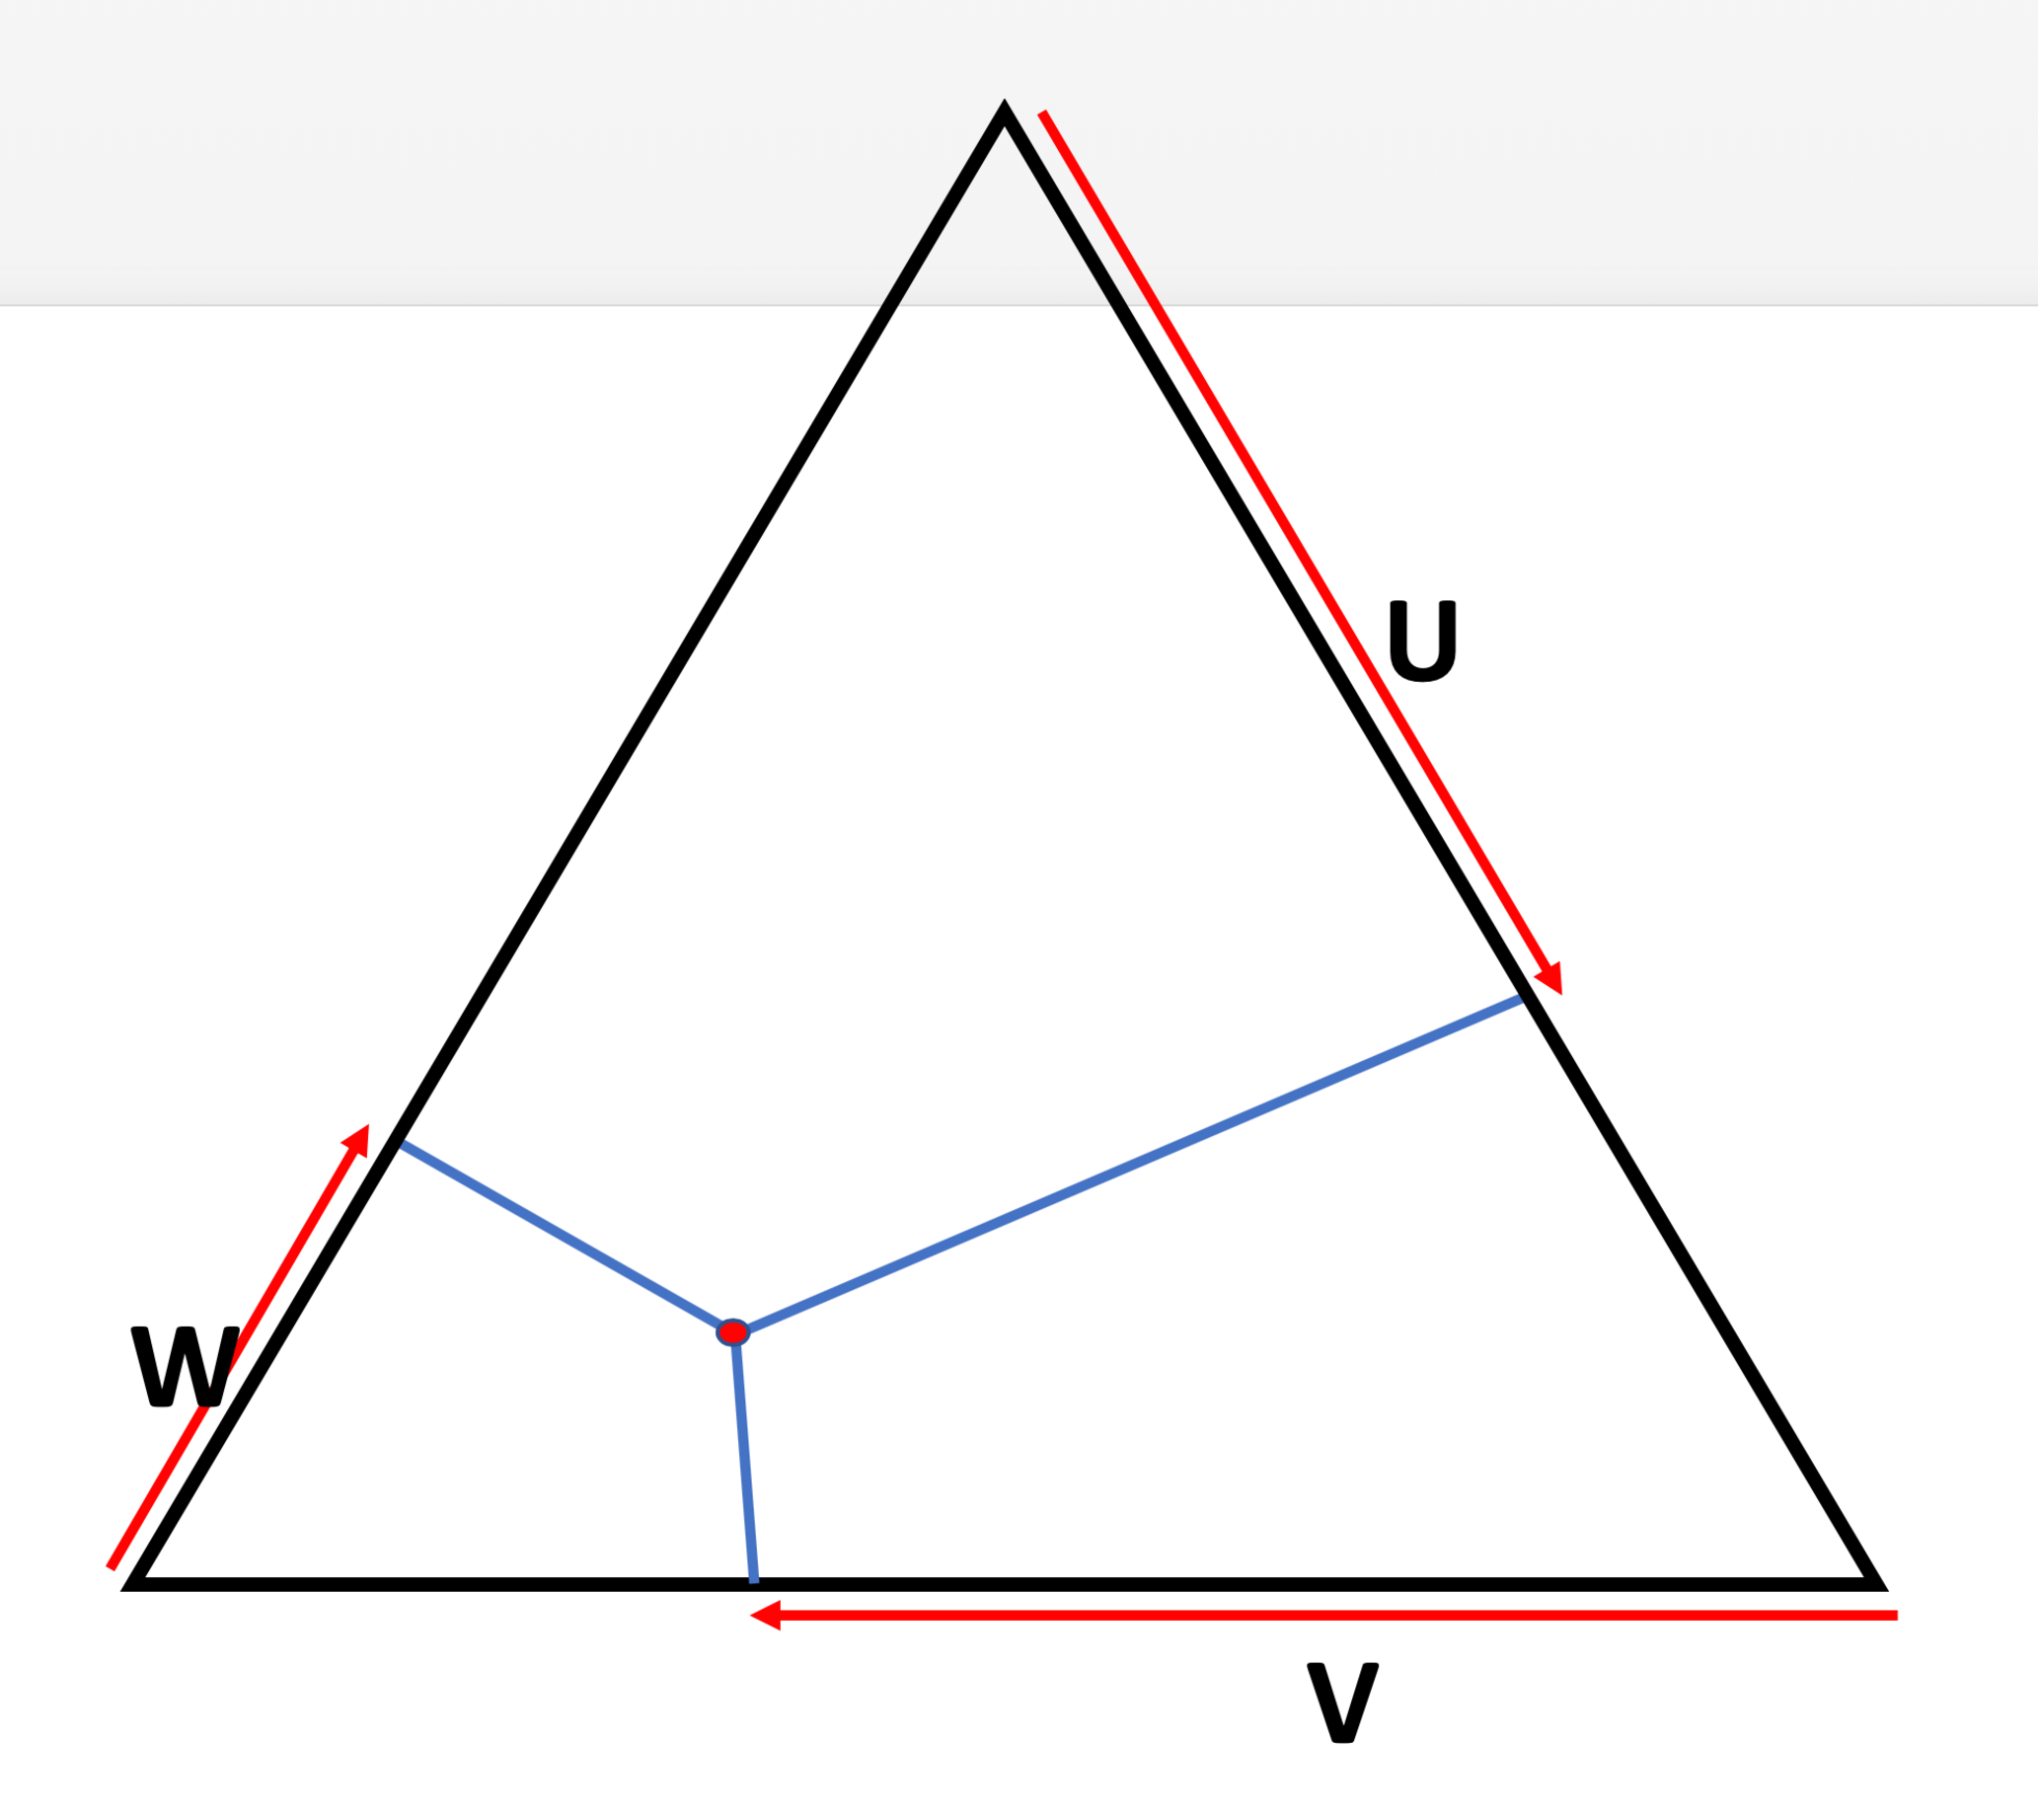
\includegraphics[width=7cm]{img/PCAL-EC.pdf}
%\includegraphics{PCA.pdf}
\caption{Cluster's reconstruction in the PCAL and EC calorimeters}
\label{fig:PCAL}
\end{center}
\end{figure} 

The PCAL and EC calorimeters are designed to detect photons and electrons. The high energy deposition in the calorimeters is one of the electron trigger parameters.
 The PCAL and EC  trigger firmware is using algorithm very close to the energy and coordinate reconstruction of the electromagnetic shower in the  off-line analysis. 
The trigger firmware is searching  for clusters in the (U,V,W) calorimeter planes and is calculating the total shower energy
and space coordinates. (see Fig.~\ref{fig:PCAL}).
The PCAL and EC detectors were calibrated before experiment in terms of energy deposition measured in MeV.
The electron trigger is using cuts on the cluster energy  in PCAL ($E_{PCAL}$) and EC ($E_{EC}$) separately and cut on the total energy deposition in both detectors $E_{Total}=E_{PCAL}+E_{EC}$.
These cuts   depend  on the beam energy and the experiment requirements and usually lie in the region 150-300 MeV for the energy sum $E_{Total}$.

Geometrical matching between the HTCC signal and position of the shower in the PCAL calorimeter helps to suppress the
random coincidence between two detectors. The trigger firmware is using the HTCC-PCAL lookup table to make a proper event selection.   

The track reconstruction in the DC system at the trigger level is very useful for the further suppression of the accidental background. 
Identifying candidates to tracks begins with  the finding track segments in superlayers in each sector in parallel. Track segments are found by comparing drift chamber hits with templates that were design to catch all tracks that are relevant for the experiment.
The segment finder may be programmed to vary the minimum number of layers in the track.  After findings the  segments the
coordinates of the track  in the superlayers are  comparing with the template track roads generated by Monte Carlo program or taken from the real data. The track candidate is tagged when the track segments are found in at least of 5  out of 6 superlayers.
The geometrical matching between track candidates and hits in the HTCC,  PCAL and EC detectors is using to strengthen the trigger performance.

The electron trigger configuration may be presented by the formula:
\begin{align*} 
 &HTCC_i(N_{phe}{>}N^{HTCC}_{min})\times\\
 & [E_{PCAL}{>}E^{PCAL}_{min})\times E_{Total}{>}E^{Total}_{min})\times  DC]_i
\end{align*}
\noindent
where index $i$ is the CLAS12 sector number, $N_{phe}$ is the number of photoelectrons detected by HTCC.  $N^{HTCC}_{min}$, 
$E^{PCAL}_{min}$, $ E^{Total}_{min}$ are the trigger parameters, and $DC$ means that  track was reconstructed by the $DC$-system. The space correlations between all detectors and coordinates of the track are implemented as well.


\subsection{Photoproduction trigger}
The photoproduction trigger is designed to select  events when scattered electron is detected by the Forward Tagger in the angular range $\theta\sim2-5$ degrees
$$
e p  \rightarrow e^\prime(detected\ by\ FT) X.
$$
\noindent
Strictly speaking it is not photoproduction process but electron scattering with  low $Q^2=4E_{beam}E'\sin^2\theta/2$.
The trigger firmware is continuously searching for the clusters developed in the FT calorimeter by electromagnetic shower and is calculating the shower energy and space coordinates. 
The cluster energy is the sum of all the
crystal energies within a 3x3 spatial array and time constraints. Once
the clustering algorithm  has identified a cluster, the
corresponding data is reported to the main trigger processor. This
includes: the timestamp, the energy, and the spatial coordinates (center
of the seed crystal). The cluster energy is not corrected for shower
leakage effects at this stage. Finally, the trigger processor makes the
trigger decision by applying further cuts to the clusters. The trigger  selection is based on lower and upper energy limits and a number of hits in the cluster. The trigger may also select events with the definite number of clusters detected by the calorimeter. 
The coincidence with the two-planes  scintillating hodoscope   located in front of the calorimeter serves to discriminate the charge particles from the high energy photons. 
It gives the possibility to select the reaction with electron and several photons in the final state, for example
$$
ep\to e'\gamma\gamma X.
$$
\noindent
The trigger system may use the  information from forward and barrel detectors to select the events with several charge or neutral particles in coincidence with the electron in the FT calorimeter. The trigger detector composition depends on the reaction under study. 

The charge particles in the forward detectors  were selected by the coincidence between TOF, PCAL and EC with the tracks reconstructed by the DC system. The space correlation between all trigger detectors are required including coordinates 
 of tracks crossing the detector's planes. The cluster-track matching is an important part of the background reduction at the trigger level. The cuts on the energy depositions in the trigger detectors are used to select charge and neutral particles. 
 
 The following trigger configuration 
 \begin{align*} 
 &FT(E^{FT}_{min}{<}E{<}E^{FT}_{max})\times\\
 & [FTOF(E{>}E^{FTOF}_{min})\times PCAL(E{>}E^{PCAL}_{min})\times  DC]_i
\end{align*}
  was used in the first CLAS12 experiments to select the reaction $ep\to e'h^{+/-}X$
 with at least one electron and one charge particle in the final state. Index i denotes the CLAS12 sector number. 
 Each detector has his own trigger energy cuts: $ E^{FT}_{min}$,  $E^{FT}_{max}$, $E^{FTOF}_{min}$ and $E^{PCAL}_{min}$.
 The space correlation between the FTOF and PCAL elements was implemented.
 The trigger rate was too high for the DAQ bandwidth so this trigger was prescaled. 

The selection of the events with at least two charge particles detected in the forward direction in different sectors was done by the trigger configuration
 \begin{align*} 
 &FT(E^{FT}_{min}{<}E{<}E^{FT}_{max})\times\\
 & [FTOF(E{>}E^{FTOF}_{min})\times  PCAL(E{>}E^{PCAL}_{min})\times   DC]_i \times \\
 & [FTOF(E{>}E^{FTOF}_{min})\times  PCAL(E{>}E^{PCAL}_{min})\times   DC]_j,
\end{align*}
 where $i$ and$j$ denote different CLAS12 sectors. This trigger selects events with electron detected by the FT calorimeter and two charged particles in the different CLAS12 sectors. 
 
 The central detectors, such as central time of flight (CTOF) and central neutral detector (CND), were used for the selection of the events with at least one  particle detected in the central detector. The following trigger configurations
 \begin{align*} 
 &FT(E^{FT}_{min}{<}E{<}E^{FT}_{max})\times\\
 & [FTOF(E{>}E^{FTOF}_{min})\times  PCAL(E{>}E^{PCAL}_{min})\times   DC]_i \times \\
 & CTOF(E{>}E^{CTOF}_{min})\end{align*}
\noindent
were used for the selection of the electron in FT, at least one charge paticle going in the forward direction and at least one particle detected in the central detectors.
In case the trigger rate is too high for the DAQ bandwidth the CND detector could be added to the coincidence chain with the space correlation between the CTOF and CND counters
 \begin{align*} 
 &FT(E^{FT}_{min}{<}E{<}E^{FT}_{max})\times PCAL(E{>}E^{PCAL}_{min})\times   DC]_i \times \\
 & CTOF(E{>}E^{CTOF}_{min})\times  CND(E{>}E^{CND}_{min}).
\end{align*}
\noindent
 As it was stated above the energy depositions in all detectors were the trigger parameters depending on the experiment requirements.


\section{$J/\psi$ meson trigger}

The special trigger was designed to detect the quasi-photoproduction of $J/\psi$-mesons
$$
ep \to e' J/\psi p'.
$$
Two decay modes are useful for the selection of the $J/\psi$ meson: $J/\psi \to e^+e^-$ and $J/\psi \to \mu^+\mu^-$.
The conventional electron and phototproduction triggers  select the $J/\psi$-meson  in case of the decay to the electron-positron pair.
But these trigger configurations don't  work  with the muons in the final state. However it was mandatory to add one more decay mode for this experiment. It will double the statistics and has no radiative tail in comparison with electron-positron pair in the final state. The CLAS12 spectrometer has no muon system. But it turns out that the selection of particles with the energy deposition in the
PCAL-EC  calorimeters close to the minimum  ionizing  value is sufficient to suppress the background from pions when the 
invariant mass of two  particles (muons or pions) is near the $J/\psi$-mass. The muons from the $J/\psi$ decay appear in the opposite CLAS12 sectors that was used in the trigger configuration  
\begin{align*} 
 & [FTOF(E{{>}}5){\times}  PCAL(15{<}E{<}60){\times} EC(60{<}E{<}120){\times}   DC]_i {\times} \\
 & [FTOF(E{{>}}5){\times}  PCAL(15{<}E{<}60){\times} EC(60{<}E{<}120){\times}   DC]_j  
\end{align*}
\noindent
The energy units are MeV. Note, that there is no requirement to search for the scattered electron at all. It gives an order of magnitude advantage in the  virtual photon flux in comparison the case when electron is detected in the FT-calorimeter.




